% This LaTeX was auto-generated from MATLAB code.
% To make changes, update the MATLAB code and export to LaTeX again.

\documentclass{article}

\usepackage[utf8]{inputenc}
\usepackage[T1]{fontenc}
\usepackage{lmodern}
\usepackage{graphicx}
\usepackage{color}
\usepackage{listings}
\usepackage{hyperref}
\usepackage{amsmath}
\usepackage{amsfonts}
\usepackage{epstopdf}
\usepackage{matlab}

\sloppy
\epstopdfsetup{outdir=./}
\graphicspath{ {./ejercicio01_images/} }

\begin{document}

\matlabtitle{Ejercicio N°1}


\begin{matlabcode}
clear;clc;
\end{matlabcode}

\begin{par}
\begin{flushleft}
Se definen simbólicas las variables
\end{flushleft}
\end{par}

\begin{matlabcode}
syms t vc(t) il(t) C L;
\end{matlabcode}

\begin{par}
\begin{flushleft}
Se plantean las ecuaciones y se obtienen las matrices de la forma generalizada
\end{flushleft}
\end{par}

\begin{matlabcode}
M=[-C 0;0 -L]
\end{matlabcode}
\begin{matlabsymbolicoutput}
M = 
    $\displaystyle \left(\begin{array}{cc}
-C & 0\\
0 & -L
\end{array}\right)$
\end{matlabsymbolicoutput}
\begin{matlabcode}
N=[0 1;-1 0]
\end{matlabcode}
\begin{matlaboutput}
N = 2x2    
     0     1
    -1     0

\end{matlaboutput}
\begin{matlabcode}
u=[0;0]; 
\end{matlabcode}

\begin{par}
$$u=\left(\matrix{0\cr0}\right)$$
\end{par}

\begin{par}
\begin{flushleft}
Se expresan las matrices de la forma normalizada
\end{flushleft}
\end{par}

\begin{matlabcode}
A=-1.*(M\N)
\end{matlabcode}
\begin{matlabsymbolicoutput}
A = 
    $\displaystyle \left(\begin{array}{cc}
0 & \frac{1}{C}\\
-\frac{1}{L} & 0
\end{array}\right)$
\end{matlabsymbolicoutput}

\begin{par}
\begin{flushleft}
Se definen las variables de estado
\end{flushleft}
\end{par}

\begin{matlabcode}
x=[vc;il]
\end{matlabcode}
\begin{matlabsymbolicoutput}
x(t) = 
    $\displaystyle \left(\begin{array}{c}
\textrm{vc}\left(t\right)\\
\textrm{il}\left(t\right)
\end{array}\right)$
\end{matlabsymbolicoutput}

\begin{par}
\begin{flushleft}
Expresando el sistema en forma diferencial
\end{flushleft}
\end{par}

\begin{matlabcode}
odes = diff(x) == A*x
\end{matlabcode}
\begin{matlabsymbolicoutput}
odes(t) = 
    $\displaystyle \left(\begin{array}{c}
\frac{\partial }{\partial t}\;\textrm{vc}\left(t\right)=\frac{\textrm{il}\left(t\right)}{C}\\
\frac{\partial }{\partial t}\;\textrm{il}\left(t\right)=-\frac{\textrm{vc}\left(t\right)}{L}
\end{array}\right)$
\end{matlabsymbolicoutput}

\begin{par}
\begin{flushleft}
Resolviendo el sistema con el comando dsolve
\end{flushleft}
\end{par}

\begin{matlabcode}
[vSol(t), iSol(t)] = dsolve(odes);
\end{matlabcode}

\begin{par}
\begin{flushleft}
\textbf{Tensión del capacitor}
\end{flushleft}
\end{par}

\begin{matlabcode}
vSol(t) = simplify(vSol(t))
\end{matlabcode}
\begin{matlabsymbolicoutput}
vSol(t) = 
    $\displaystyle C_5  e^{\frac{t \sqrt{-C L}}{C L}} +C_6  e^{-\frac{t \sqrt{-C L}}{C L}} $
\end{matlabsymbolicoutput}

\begin{par}
\begin{flushleft}
\textbf{Corriente del inductor}
\end{flushleft}
\end{par}

\begin{matlabcode}
iSol(t) = simplify(iSol(t))
\end{matlabcode}
\begin{matlabsymbolicoutput}
iSol(t) = 
    $\displaystyle \frac{e^{-\frac{t \sqrt{-C L}}{C L}}  {\left(C_6 -C_5  e^{\frac{2 t \sqrt{-C L}}{C L}} \right)} \sqrt{-C L}}{C}$
\end{matlabsymbolicoutput}

\begin{par}
\begin{flushleft}
Reemplazando los valores de R, L y C
\end{flushleft}
\end{par}

\begin{matlabcode}
clear C L;
syms C1 C2;
R=1;L=1;C=1;
A=subs(A);
\end{matlabcode}

\begin{par}
\begin{flushleft}
Las ecuaciones diferenciales son
\end{flushleft}
\end{par}

\begin{matlabcode}
odes = diff(x) == A*x
\end{matlabcode}
\begin{matlabsymbolicoutput}
odes(t) = 
    $\displaystyle \left(\begin{array}{c}
\frac{\partial }{\partial t}\;\textrm{vc}\left(t\right)=\textrm{il}\left(t\right)\\
\frac{\partial }{\partial t}\;\textrm{il}\left(t\right)=-\textrm{vc}\left(t\right)
\end{array}\right)$
\end{matlabsymbolicoutput}

\begin{par}
\begin{flushleft}
Definiendo las condiciones iniciales y tiempo de simulacion
\end{flushleft}
\end{par}

\begin{matlabcode}
v0=2;
i0=1;
ti=0;
tf=4*pi;
Xant=[v0;i0];
constantes=x(0)==Xant;
[vSol(t), iSol(t)] = dsolve(odes,constantes)
\end{matlabcode}
\begin{matlabsymbolicoutput}
vSol(t) = 
    $\displaystyle \sqrt{5} \cos \left(t+\textrm{atan}\left(2\right)\right)$
iSol(t) = 
    $\displaystyle \sqrt{5} \cos \left(t-\textrm{atan}\left(\frac{1}{2}\right)\right)$
\end{matlabsymbolicoutput}


\begin{matlabcode}
clf;
fplot(iSol,[ti,tf],'-g')
hold on
fplot(vSol,[ti,tf],'-b')
title('Respuesta temporal')
xlabel('tiempo [s]')
ylabel('Voltaje [V] Corriente [A]')
legend({'Corriente IL1','Voltaje VC1'})
hold off
\end{matlabcode}
\begin{center}
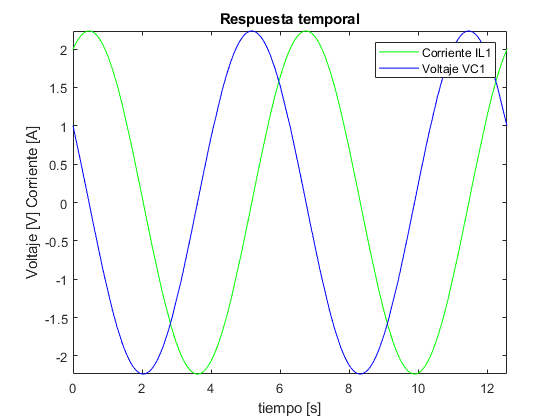
\includegraphics[width=\maxwidth{56.196688409433015em}]{figure_0_00}
\end{center}


\begin{matlabcode}
fplot(iSol,vSol)
title('Phase Portrait')
xlabel('Corriente [A]')
ylabel('Voltaje [V]')
hold off
\end{matlabcode}
\begin{center}
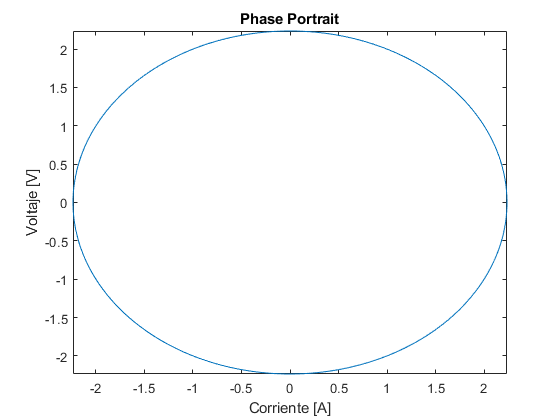
\includegraphics[width=\maxwidth{56.196688409433015em}]{figure_1_00}
\end{center}

\end{document}
